\subsection{Use cases}
Use cases beskriver hvordan en eventuel spiller interagere med spillet. 
\begin{figure}[h]
    \centering
    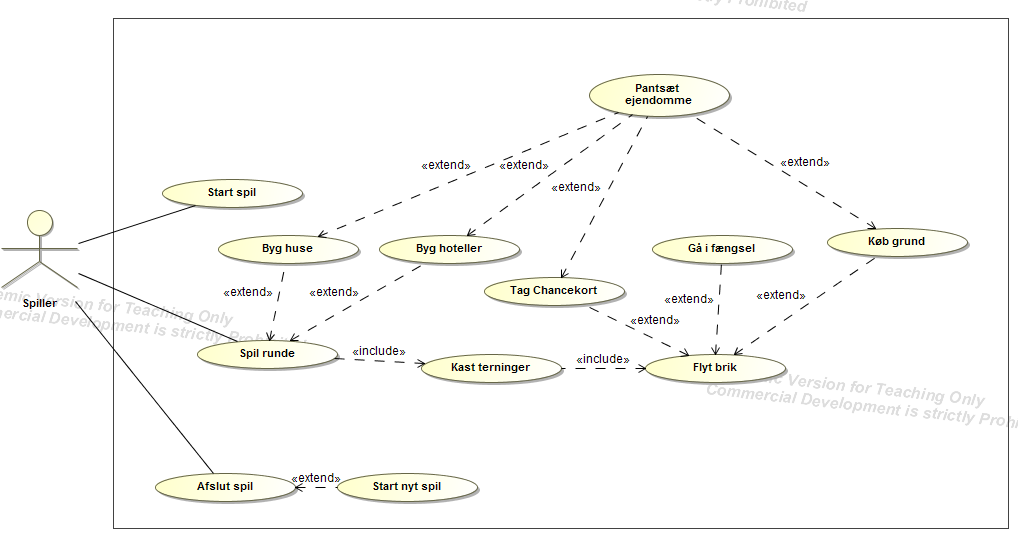
\includegraphics[width=\textwidth]{sources/5_analyse/UseCaseDiagram.PNG}
    \caption{Use case diagram}
    \label{fig:UC1}
\end{figure}

Ud fra diagrammet er der blevet udvalgt nogle kritiske use cases, som er afgørende i forhold til hvordan spillet spilles. 

\begin{itemize}
    \item Start spil
    \item Flyt brik
    \item Køb grund
    \item Gå i fængsel
    \item Tag chancekort
    \item Afslut spil
\end{itemize}

\newpage
\subsection{Use case beskrivelser}

\begin{center}
\begin{longtable}{|l|p{11cm}|}
\hline
Navn &  UC1 - Start spil\\
\hline
Short description & Spillerne starter spillet på computeren \\
\hline
Precondition & Programmet er installeret på computeren \\
\hline
Postcondition & Spillet er startet med de valgte antal spillere \\
\hline
Fejlsituationer & Ugyldigt antal spillere \\
\hline
Status i tilfælde af fejl & Spillet starter ikke \\
\hline
Aktører & Spiller \\
\hline
Udløser & Spillerne vil gerne spille spillet \\
\hline
Standard process &  
\begin{minipage}[t]{1\textwidth}
  \begin{enumerate}
      \item Spillet startes op på computeren
      \item Der vælges et antal spillere fra 2-6
      \item Der vælges navn for spillerne
      \begin{itemize}
          \item Spiller 2-6 vælger navn 
          \newline
          \emph{gentag indtil alle spiller har valgt navn}.
      \end{itemize}
      \item Der vælges farve for spillerne
      \begin{itemize}
          \item Spiller 2-6 vælger farve 
          \newline
          \emph{gentag indtil alle spiller har valgt en farve}.
      \end{itemize}
      \item Der vælges en brik til alle spillerne
      \begin{itemize}
          \item Spiller 2-6 vælger brik 
          \newline
          \emph{gentag indtil alle spiller har valgt en brik}.
      \end{itemize}
      \item Spillet starter med de valgte navne, farver og brikker.\vspace{0.5cm}
  \end{enumerate} 
  \end{minipage}
\\
\hline
Alternativ process & 
\begin{minipage}[t]{1\textwidth}
 \begin{itemize}
 \vspace{0.5cm}
     \item Der indtaster mindre eller flere spillere end 2-6
        \begin{enumerate}
            \item Spillet giver en fejlbesked
            \item Spilleren ændrer antal spillere
            \item forsætter fra 2. i hoveddelen
        \end{enumerate}
    \item Der vælges en forkert brik, eller en brik der er optaget
    \begin{enumerate}
        \item Spillet giver en fejlbesked
        \item Spilleren vælger en anden brik
        \item fortsætter fra 7. i hoveddelen
    \end{enumerate}
 \end{itemize}
\end{minipage}

\\
\hline
\end{longtable}
\end{center}



\begin{center}
\begin{longtable}{|l|p{11cm}|}
\hline
Navn &  UC2 - Flyt brik\\
\hline
Short description & Den nuværende spiller kaster terningerne og flytter sin brik \\
\hline
Precondition & Det er spillerens tur \\
\hline
Postcondition & Spilleren har taget sin tur, og turen er gået videre til den næste spiller \\
\hline
Fejlsituationer & Ingen \\
\hline
Status i tilfælde af fejl & Spilleren tager ikke sin tur \\
\hline
Aktører & Spiller \\
\hline
Udløser & Det er spillerens tur \\
\hline
Standard process &  
\begin{minipage}[t]{1\textwidth}
  \begin{enumerate}
      \item Spilleren kaster terningerne.
      \item Spilleren flytter sin brik fra det nuværende felt \newline til det næste felt.
      \begin{itemize}
          \item Spilleren lander på en grund.\newline
          \emph{Se alternativ process.} 
          \item Spilleren lander på besøg i fængsel.\newline
          \emph{Se alternativ process.}
          \item Spilleren lander på gå i fængsel.\newline
          \emph{Se alternativ process.}
          \item Spilleren lander på Prøv lykken.\newline
          \emph{Se alternativ process.}
          \item Spilleren lander på Parkering.\newline
          \emph{Se alternativ process.}
          \item Spilleren lander på et beskatningsfelt.\newline
          \emph{Se alternativ process.}
      \end{itemize}
      \item Passerede spilleren start?
      \begin{itemize}
          \item Modtag 4000. 
      \end{itemize}
      \item Slog spilleren to ens?
      \begin{itemize}
          \item Gå til trin 1.
      \end{itemize}
      \item Turen går videre til den næste spiller.\vspace{0.5cm}
  \end{enumerate} 
  \end{minipage}
\\
\hline
Alternativ process & 
\begin{minipage}[t]{1\textwidth}
 \begin{itemize}
     \item Grund
     \begin{enumerate}
         \item Hvis ingen ejer grunden,\newline vil spilleren købe grunden? (Se UC3)
         \item Hvis en anden spiller ejer grunden, betal leje.
         \item Hvis spilleren selv ejer grunden, ingenting. \newline (Gå til trin 3. i hoveddel)
     \end{enumerate}
     \item Besøg i fængsel
     \begin{enumerate}
         \item Der sker ingenting
         \item Gå til trin 3. i hoveddel.
     \end{enumerate}
     \item Gå i fængsel
     \begin{enumerate}
         \item Flyt spillerens brik i fængsel
         \item Gå til trin 5. i hoveddel.
     \end{enumerate}
     \item Prøv lykken
     \begin{enumerate}
         \item Tag chancekort 
         \item udfør chancekort.
         \item Gå til trin 3. i hoveddel.
     \end{enumerate}
     \item Parkering
     \begin{enumerate}
         \item Gå til trin 3. i hoveddel.
     \end{enumerate}
     \item Beskatningsfelt
     \begin{enumerate}
         \item Betal skat
         \item Gå til trin 3. i hoveddel.
     \end{enumerate}
 \end{itemize}
\end{minipage}

\\
\hline
\end{longtable}
\end{center}


\begin{center}
\begin{longtable}{|l|p{11cm}|}
\hline
Navn &  UC3 - Gå i fængsel\\
\hline
Short description & Spilleren skal sættes i fængsel \\
\hline
Precondition & Spilleren er landet på fængslet eller har trukket et ‘gå i fængsel’ chancekort. \\
\hline
Postcondition & Spilleren er i fængsel \\
\hline
Fejlsituationer & Spilleren ejer et ‘undgå fængsel’ chancekort. \\
\hline
Status i tilfælde af fejl & Spilleren mister sit kort og undgår fængsel. \\
\hline
Aktører & Spiller \\
\hline
Udløser & 1. Spilleren er landet på fængslet.
2. Spilleren har trukket et ‘gå i fængsel’ chancekort.
 \\
\hline
Standard process &  
\begin{minipage}[t]{1\textwidth}
  \begin{enumerate}
      \item Spilleren lander på fængsel-feltet.\newline
      \emph Se alternativ process\
      \begin{itemize}
          \item Spilleren har trukket et 'gå i fængsel' chancekort
      \end{itemize}
      \item Passerede spilleren start?
      \begin{itemize}
          \item Modtag 4000. 
      \end{itemize}
      \item Slog spilleren to ens?
      \begin{itemize}
          \item Gå til trin 1.
      \end{itemize}
      \item Turen går videre til den næste spiller.\vspace{0.5cm}
  \end{enumerate} 
  \end{minipage}
\\
\hline
Alternativ process & 
\begin{minipage}[t]{1\textwidth}
 \begin{itemize}
     \item Grund
     \begin{enumerate}
         \item Hvis ingen ejer grunden,\newline vil spilleren købe grunden? (Se UC3)
         \item Hvis en anden spiller ejer grunden, betal leje.
         \item Hvis spilleren selv ejer grunden, ingenting. \newline (Gå til trin 3. i hoveddel)
     \end{enumerate}
     \item Besøg i fængsel
     \begin{enumerate}
         \item Der sker ingenting
         \item Gå til trin 3. i hoveddel.
     \end{enumerate}
     \item Gå i fængsel
     \begin{enumerate}
         \item Flyt spillerens brik i fængsel
         \item Gå til trin 5. i hoveddel.
     \end{enumerate}
     \item Prøv lykken
     \begin{enumerate}
         \item Tag chancekort 
         \item udfør chancekort.
         \item Gå til trin 3. i hoveddel.
     \end{enumerate}
     \item Parkering
     \begin{enumerate}
         \item Gå til trin 3. i hoveddel.
     \end{enumerate}
     \item Beskatningsfelt
     \begin{enumerate}
         \item Betal skat
         \item Gå til trin 3. i hoveddel.
     \end{enumerate}
 \end{itemize}
\end{minipage}

\\
\hline
\end{longtable}
\end{center}


\newpage
\begin{center}
\begin{longtable}{|l|p{11cm}|}
\hline
Navn &  UC5 - Tag chancekort\\
\hline
Short description & Den nuværende spiller tager et chancekort fra bunken og retter sig efter beskrivelsen. \\
\hline
Precondition & Spilleren er landet på et "Prøv lykken" felt \\
\hline
Postcondition & Spilleren har efterlevet chancekortets beskrivelse, og turen er gået videre til den næste spiller \\
\hline
Fejlsituationer & Ingen \\
\hline
Status i tilfælde af fejl & Spilleren modtager ikke chancekort. \\
\hline
Aktører & Spiller \\
\hline
Udløser & Spilleren er landet på et "Prøv lykken" felt \\
\hline
Standard process &  
\begin{minipage}[t]{1\textwidth}
  \begin{enumerate}
      \item Spilleren lander på et felt af typen "Prøv lykken".
      \item Spilleren trækker et tilfældigt chancekort, af typen:
      \begin{itemize}
          \item Betal penge til banken.\newline
          \emph{Se alternativ process.} 
          \item Modtag penge fra banken.\newline
          \emph{Se alternativ process.}
          \item Modtag penge fra spillere.\newline
          \emph{Se alternativ process.}
          \item Ryk felt.\newline
          \emph{Se alternativ process.}
          \item Gå i fængsel.\newline
          \emph{Se alternativ process.}
      \end{itemize}
      \item Passerede spilleren start?
      \begin{itemize}
          \item Modtag 4000. 
      \end{itemize}
      \item Slog spilleren to ens?
      \begin{itemize}
          \item Gå til trin 1 i "Flyt brik". 
      \end{itemize}
      \item Turen går videre til den næste spiller.\vspace{0.5cm}
  \end{enumerate} 
  \end{minipage}
\\
\hline
Alternativ process & 
\begin{minipage}[t]{1\textwidth}
 \begin{itemize}
     \item Betal penge til banken
     \begin{enumerate}
         \item Spilleren betaler det beskrevne beløb til banken.
         \item Hvis spilleren ikke har det beskrevne beløb \newline i sin konto udgår han af spillet.
     \end{enumerate}
     \item Modtag penge fra banken
     \begin{enumerate}
         \item Spilleren modtager det beskrevne beløb \newline fra banken.
     \end{enumerate}
     \item Modtag penge fra spillere
     \begin{enumerate}
         \item Spilleren modtager det beskrevne beløb \newline fra sine medspillere.
         \item Hvis medspillerene ikke har det beskrevne \newline beløb i sin konto udgår de af spillet.
     \end{enumerate}
     \item Ryk felt
     \begin{enumerate}
         \item Spilleren rykker det angivne antal felter. 
     \end{enumerate}
     \item Gå i fængsel
     \begin{enumerate}
         \item Spilleren placeres på "I fængsel" feltet.
     \end{enumerate}
     
 \end{itemize}
\end{minipage}

\\
\hline
\end{longtable}
\end{center}

\newpage
\begin{center}
\begin{longtable}{|l|p{11cm}|}
\hline
Navn &  UC6 - Afslut spil\\
\hline
Short description & Spillet har fået en vinder og spillet afsluttes \\
\hline
Precondition & Der er kun en spiller tilbage \\
\hline
Postcondition & Spillerene bliver tilbudt at spille igen \\
\hline
Fejlsituationer & Ingen \\
\hline
Status i tilfælde af fejl & Spillet afsluttes ikke \\
\hline
Aktører & Spiller \\
\hline
Udløser & Alle spillere pånær én er udgået \\
\hline
Standard process &  
\begin{minipage}[t]{1\textwidth}
  \begin{enumerate}
      \item Der er kun en spiller tilbage
      \item Den sidste spiller kåres til vinder af spillet
      \item Spillerne bliver præsenteret for et valg
      \begin{itemize}
          \item Spil igen 
          \newline
          \item Afslut spil 
          \newline
      \end{itemize}
  \end{enumerate} 
  \end{minipage}
\\
\hline
Alternativ process & 
\begin{minipage}[t]{1\textwidth}
 \begin{itemize}
 \vspace{0.5cm}
     \item Spil igen
        \begin{enumerate}
            \item Spillet startes forfra (se UC1)
        \end{enumerate}
    \item Afslut spil
    \begin{enumerate}
        \item Programmet lukkes
    \end{enumerate}
 \end{itemize}
\end{minipage}

\\
\hline
\end{longtable}
\end{center}